\documentclass[final, letterpaper, square, comma, numbers, sort&compress]{elsarticle}
\usepackage[utf8]{inputenc}
\usepackage[
    % margin=1in
    top=1in,
    bottom=0.7in,
    left=1in,
    right=1in,
    %footskip=0.5in, % FIXME: temp fix
    footnotesep=0.3in,
    % showframe % Uncomment to show frames around the margins for debugging purposes
]{geometry}

\usepackage{hyperref}
\hypersetup{
	% colorlinks=true, % Whether to color the text of links
	% urlcolor=black, % Color for \url and \href links
	% linkcolor=black, % Color for \nameref links
	% citecolor=black, % Color of reference citations
        hidelinks,
        pdfauthor={R. Ranjan; J. Wilson; M. Barisik; V. Ramanuj; R. Sankaran;},
        pdftitle={Effects of Operating Conditions on the Gas-Phase Decomposition of MTS/H2 during Chemical Vapor Infiltration of SiC} % these lines are nessesary to avoid hyperref throwing errors from pulling the newline in the given frontmatter title section
}

\usepackage{graphicx}
\graphicspath{{figures/}}
\usepackage{amssymb}
\usepackage{amsmath}
\usepackage{array}
\usepackage[bottom]{footmisc}

\journal{Energy Policy} % FIXME

\begin{document}

\begin{frontmatter}


%% Title, authors and addresses
\title{Effects of Operating Conditions on the Gas-Phase Decomposition of \\ MTS/H$_2$ during Chemical Vapor Infiltration of SiC }

\author[1]{R.~Ranjan\corref{cor1}}
\ead{reetesh-ranjan@utc.edu}
\author[1]{J.~Wilson}
\author[1]{M.~Barisik}
\author[2]{V.~Ramanuj}
\author[2]{R.~Sankaran}
\cortext[cor1]{Corresponding author}

\address[1]{Department of Mechanical Engineering, The University of Tennessee Chattanooga \\
615 McCallie Avenue, Chattanooga, TN 37403, USA}
\address[2]{Computational Sciences and Engineering Division, Oak Ridge National Laboratory \\
1 Bethel Valley Rd., Oak Ridge, TN 37831, USA}

\begin{abstract}
The quality of the silicon carbide (SiC) matrix composite, which has excellent thermo-mechanical properties, fabricated by the well-established chemical vapor infiltration (CVI) process, depends upon the gas-phase decomposition of the employed precursor and the subsequent heterogeneous reactions at the deposition surface. The decomposition process is primarily affected by the operating parameters such as temperature, pressure, gradient of pressure and temperature, and the composition of the incoming gas-phase reactants. In this study, we perform plug flow reactor (PFR) analysis to examine the effects of operating parameters on the decomposition of the mixture of methyltrichlorosilane (MTS) and hydrogen ($\rm H_2$), a widely used precursor for the manufacturing of SiC matrix composite using the CVI process. The PFR analysis is performed using three chemical mechanisms of increasing degree of complexity, which include globally reduced (1 step and 5 species), moderately complex (30 steps and 20 species), and detailed (103 steps and 42 species) mechanisms. First, we discuss the reduction strategy to obtain the moderately complex mechanism from the detailed one and assess the performance of the three mechanisms by comparing PFR results at atmospheric pressure with reference experimental and numerical results. Afterward, the PFR analysis is performed using these mechanisms at conditions relevant to CVI. These include a range of temperature (1100 K to 1600 K), pressure (5 Torr to 100 Torr), temperature gradient (-190 K/m to -19 K/m), and pressure gradient (-7.7 Torr/m to -0.97 Torr/m). The analysis of the results pertaining to the decomposition of MTS and production of several intermediate reactive species shows that the decomposition of MTS is more sensitive to temperature and its gradient than pressure or pressure gradient. The effects of the ratio of MTS and H2 in the incoming mixture (0.05 to 0.2) are examined by considering isothermal and temperature-gradient conditions. The results show enhanced decomposition of MTS in the case with the presence of a temperature gradient for the same mixture composition, and a nonlinear dependence of the decomposition of MTS and production of intermediates and byproducts on the incoming mixture composition. The present study also showed that the moderately complex chemical kinetics show good agreement with the detailed mechanism, whereas the globally reduced chemical mechanism yielded inaccurate results, thus implying that the moderately complex mechanism can be used while performing detailed three-dimensional modeling of the CVI process.
\end{abstract}

\begin{keyword}
Chemical vapor infiltration \sep silicon carbide \sep methyltrichlorosilane \sep plug flow reactor \sep chemical mechanisms
\end{keyword}

\end{frontmatter}

\let\thefootnote\relax\footnote{Notice: This manuscript has been authored by UT-Battelle, LLC, under contract DEAC05-00OR22725 with the US Depart-ment of Energy (DOE). The US government retains and the publisher, by accepting the article for publication, acknowledges that the US government retains a nonexclusive, paid-up, irrevocable, worldwide license to publish or reproduce the published form of this manuscript, or allow others to do so, for US government purposes. DOE will provide public access to these results of federally sponsored research in accordance with the DOE Public Access Plan (\ttfamily \href{http://energy.gov/downloads/doe-public-access-plan}{http://energy.gov/downloads/doe-public-access-plan}).}

\section{Introduction}
\label{S:1}

Materials that can withstand high-temperature environments are required in many engineering applica- tions such as nuclear reactors, automotive, spacecraft, aircraft components, furnace linings, power electronics,
and cutting and grinding tools. Such materials include metals and alloys (titanium alloys, tungsten, molyb- denum), ceramics (alumina, silicon carbide (SiC), graphite), and composites (ceramic matrix composites, carbon-carbon composites)~\cite{Meetham1991,Tressler1999,Belmonte2006,Fahrenholtz2014,BarCohen2014}. SiC is one such material, which has excellent properties such as high strength, high thermal conductivity, low thermal expansion, chemical inertness, and good thermal shock strength~\cite{Levinshtein2001,Hironaka2002,Snead2007,Presser2008}. However, it also tends to have a low toughness~\cite{Padture1994,Mulla1994,Cao1995}, which has motivated interest in high purity and high quality SiC fiber-reinforced matrix composites~\cite{Naslain1995,Prewo1989,Besmann1991,Wang1996,Prouhet1994,Zhu1999,Liu2023}. In such composites, a SiC matrix is deposited within a fiber preform composed of high-purity, near-stoichiometric SiC fiber. Such an approach leads to a better fracture toughness property while still having a similar performance under high thermal- loading conditions. The deposition of the SiC matrix composites depends upon the operating conditions, which affect the gas-phase decomposition and the subsequent heterogeneous surface reactions on the fiber preform. The present study examines the effects of operating conditions on the gas-phase decomposition of the precursor and the production of intermediate reactive species during SiC matrix deposition.


SiC matrix composites can be fabricated using approaches such as melt infiltration~\cite{Xu1999,DiCarlo2005}, polymer infiltration and pyrolysis~\cite{Sirieix1990, Kohyama2000}, and chemical vapor infiltration (CVI)~\cite{Sayano1999,Lamon2005,Deck2013}. Past studies have shown that CVI is a reliable approach to obtain a very high-purity SiC matrix composite~\cite{Lamon2005,Katoh2014}. During the CVI process, a SiC precursor is introduced into a chamber in the gas phase, which diffuses into the fiber preform and chemically reacts, forming a SiC matrix within the sample. There are two major challenges associated with the CVI process, which affect the overall quality of the resultant matrix composite. The first challenge is associated with the processing time. While CVI produces a very high-purity matrix, as the deposition process is dependent on the diffusion of reactants into the fiber preform, ideally, a slow reaction rate is desirable to ensure uniform transport of reactants throughout the preform. However, with a slower reaction rate, the processing time gets longer, which can affect the quality of the resulting composite. For example, high porosity can be observed, and filling of inter-tow sharp and large pores can be a challenge while keeping the processing times low~\cite{Liu2021}. Therefore, modifications have been considered to the conventional CVI process~\cite{Lamon2005,Probst1999}. These include thermal-gradient CVI~\cite{Stinton1986}, pressure-gradient CVI (forced flow CVI)~\cite{Deck2013}, pressure-pulsed CVI~\cite{Naslain2001}, and whisker-growing assisted CVI~\cite{Oh2001}. The second challenge is related to the dependence of the quality of the SiC deposition on the gas-phase decomposition of the precursor that is used during the process. Note that the precursor decomposition and production of the reactive intermediates directly affect the heterogeneous surface reactions and can also affect the overall processing time. This particular challenge can be addressed by studying the effects of operating conditions on the decomposition of the precursor used for the CVI of SiC matrix composite, which is the major focus of this study.

Some of the commonly used precursors for the fabrication of SiC through the CVI process include methyltrichlorosilane ($\rm CH_3SiCl_3$), hereafter referred to as MTS, silane ($\rm SiH_4$) along with hydrocarbons such as methane ($\rm CH_4$), dichloromethylsilane ($\rm CH_3SiHCl_2$), and hexamethyldisilane ($\rm (CH_3)_6Si_2$)~\cite{Noda1992,Naslain2006,Lazzeri2012}. Out of these, MTS is widely used as it yields a perfect stoichiometry (1:1 Si:C), leading to high-purity SiC with minimal free carbon or silicon~\cite{Lamon2005}. In addition, its decomposition characteristics can be controlled by varying operating temperature (800 to 1000 $^o$C) and pressure (5 to 100 Torr) conditions, and the ratio of MTS to hydrogen ($\rm H_2$) in the incoming mixture. Note that MTS is used as a precursor along with $\rm H_2$ as the carrier gas, which in turn can suppress free carbon formation and reduce volatile intermediates such as $\rm SiCl_4$~\cite{Lazzeri2012}. Therefore, in this study, we study the decomposition characteristics of MTS, which can lead to the production of several intermediate reactive species such as $\rm CH_4$, HCl, $\rm SiCl_4$, $\rm SiHCl_3$, etc., that in turn affect the deposition process at the preform surface where heterogeneous reactions occur.

The computational study of CVI of SiC matrix composite can be carried out using techniques with varying levels of fidelity and computational cost, which include, computational fluid dynamics (CFD)~\cite{Streitwieser2006,Ramadan2018,Cha2022,Ramanuj2022}, direct simulation Monte Carlo (DSMC)~\cite{Deck2013,Deck2012}, or plug-flow reactor (PFR)~\cite{Dang2022}. For example, while CFD can simulate large-scale fabrication systems and account for transport and diffusion processes, it faces challenges in accurate modeling of the matrix infiltration process, where the transport of the reactants occurs through the fiber preform, leading to Knudsen numbers much larger than unity. To this end, the DSMC technique can be employed, although it is computationally expensive for the simulation of large-scale fabrication systems. While using either of these techniques, accurate modeling of chemical kinetics is pivotal to the accuracy of the prediction of the gas-phase decomposition and subsequent deposition through the heterogeneous surface reactions on the fiber preform. However, due to computational complexities associated with detailed chemical kinetics, often simplified chemical mechanisms are employed while using CFD and DSMC techniques~\cite{Deck2012,Mollick2017,Ogawa2023}, which tend to yield inaccurate results. Therefore, there is a need to have reliable yet affordable chemical mechanisms that can accurately predict the gas-phase decomposition and subsequent heterogeneous reactions during CVI of SiC. In this study, we employ a plug-flow reactor (PFR) as the computational technique, which can efficiently account for detailed chemical kinetics~\cite{Papasouliotis1994,Roman1995,Bammidipati1996,Norinaga2008} to study the decomposition of MTS under different operating conditions. In a PFR, a steady flow field within an axial duct is modeled, where the flow in the transverse direction is considered to be completely homogeneous.

The key objective of this study is to first establish a PFR setup, and then to use the setup to examine the effects of operating conditions on the gas-phase decomposition of MTS and production of intermediate reactive species such as $\rm CH_4$, HCl, $\rm SiHCl_3$, $\rm SiCl_2$, and $\rm SiCl_4$ under CVI-relevant conditions. Past studies using PFR have primarily focused on the development and assessment of chemical kinetics, and therefore, the present study will complement the findings of such studies. Along with the detailed kinetics, we also assess the performance of two other chemical mechanisms, which can be potentially used with CFD and DSMC simulations. The three chemical mechanisms include detailed (103 steps and 43 species)~\cite{Ge2007A,Ge2007B,Ge2010}, moderately complex reduced (30 steps and 20 species), and globally reduced (1 step and 5 species)~\cite{Mousavipour2004} mechanisms. The moderately complex mechanism is obtained using a reduction technique (discussed later) in the present study. To examine the decomposition of MTS in the presence of $\rm H_2$, we consider different CVI reactor conditions. Apart from considering a range of operating temperatures (1100 K to 1600 K) and pressures (5 Torr to 100 Torr), we also examine the effects of a range of temperature gradients (-190 K/m to -19 K/m), and pressure gradients (-7.7 Torr/m to -0.97 Torr/m). Past studies have also shown that the decomposition of MTS is affected by the composition, i.e., molar ratio of MTS/$\rm H_2$ ($\beta$)~\cite{Peng2021}. Therefore, the effects of variation in $\beta$ (0.05 to 0.2) are also examined after identifying optimal operating temperature and pressure conditions. 

This article is arranged as follows. The details for the computational setup and the employed numerical methodology are presented in Section 2. In Section 3, an assessment of the PFR-based computational strategy is performed by comparing the results with reference data from the literature. The results of this study are discussed in Section 4. Finally, the key outcomes of this study are summarized in Section 5.

\section{Setup and Approach}
\label{S:2}

\begin{figure}[t]
\centering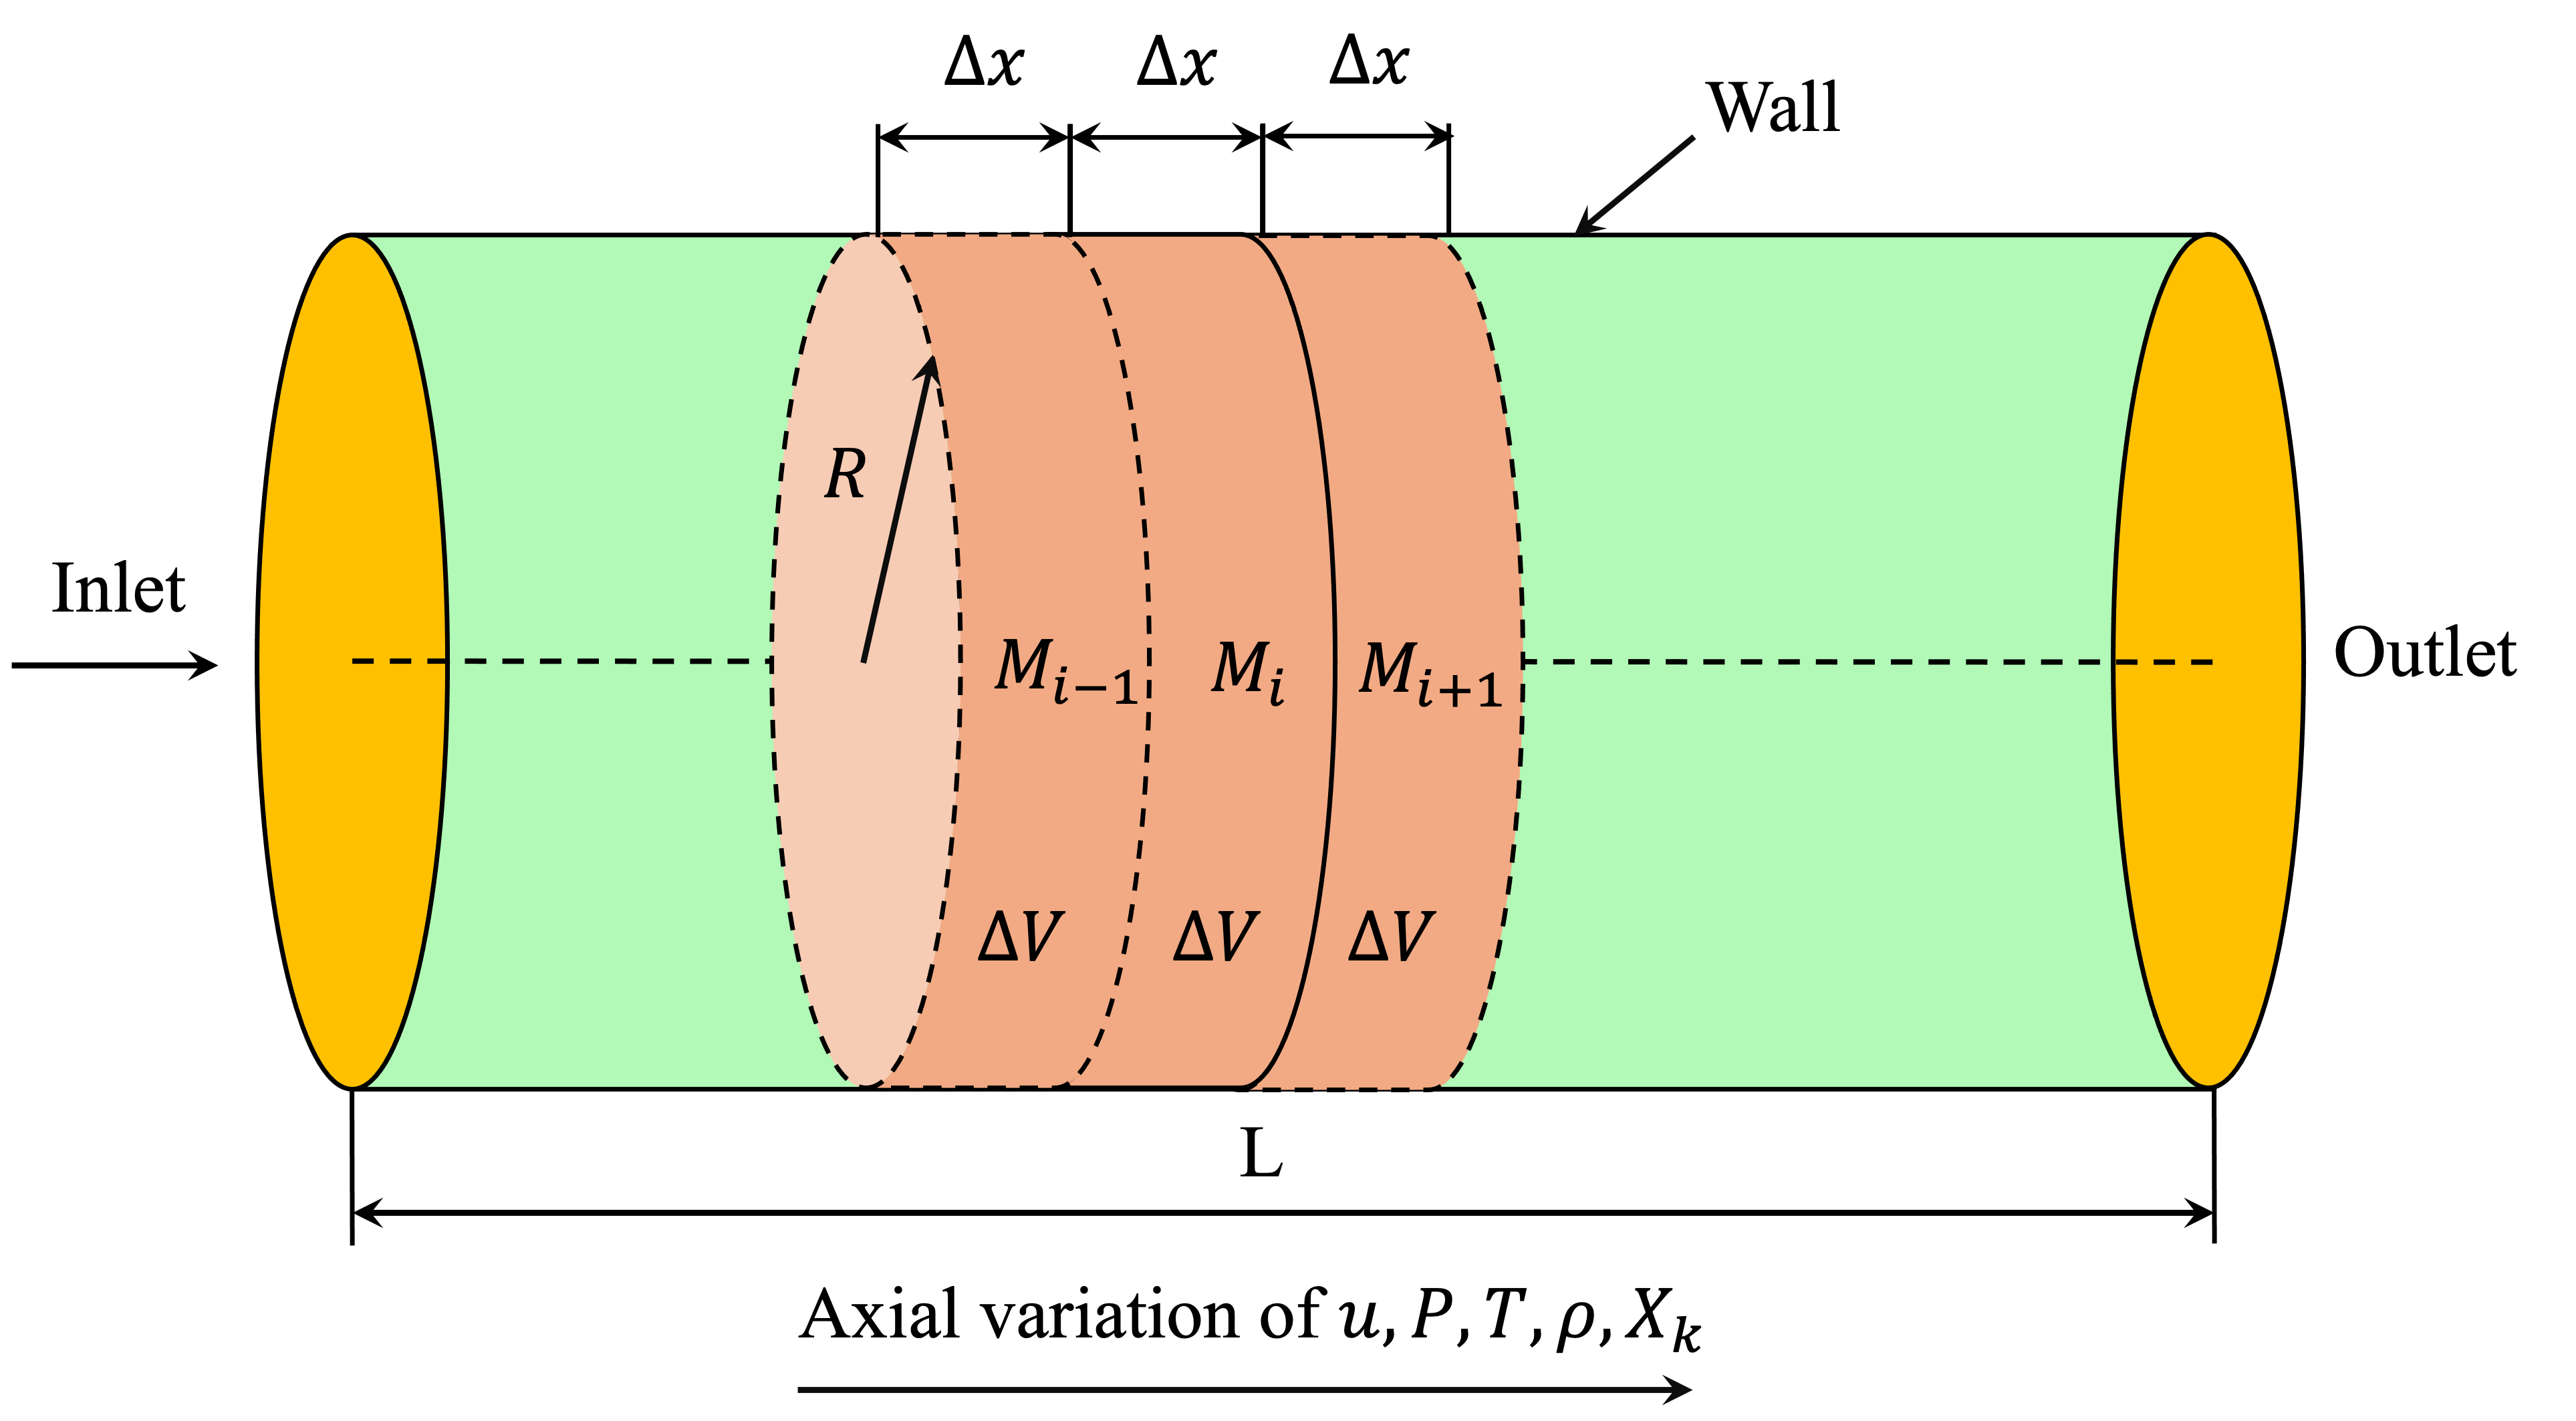
\includegraphics[width=0.61\textwidth]{PFR-schematic.png}
\caption{Schematic of a plug flow reactor-based representation of the hot-wall CVI reactor configuration. Here, $M_i$ denotes the $i^{th}$ plug along the axial ($x$) direction, and $\Delta x$, $\Delta V$, and $R$ denote the axial length, volume, and radius of the plug, respectively.}
\label{PFR-schematic}
\end{figure}

In this section, we first describe the details of the CVI reactor configuration. Afterward, the computational method is described. Finally, the details of the chemical mechanisms used in this study are presented.

\subsection{Details of the Setup}
\label{S:2.1}
We consider a cylindrical hot-wall flow CVI reactor configuration. A schematic of this reactor is shown in Fig. \ref{PFR-schematic}. The dimensions of the reactor follow a past study \cite{Dang2022}. The axial extent of the cylindrical reactor is $L = 0.52 \rm\ m$, and the inner radius is $R = 0.0048 \rm\ m$. At the inlet of the reactor, a premixed mixture of MTS, $\rm H_2$, and Ar enters at pressure $P$ and temperature $T$. The molar composition at the inlet of the reactor is 95\% Ar and 5\% mixture of MTS and $\rm H_2$. The ratio of molar composition of MTS and $\rm H_2$ is specified to be $\beta$, which is varied in this study from 0.05 to 0.2.

\subsection{Computational Approach}
\label{S:2.2}
The chemically reacting flow in the CVI reactor is simulated using a laminar PFR model. Such an approach has been followed in past studies for modeling the flow within CVD and CVI reactors \cite{Dang2022,Roman1995,Bammidipati1996}. A schematic of PFR is shown in Fig. \ref{PFR-schematic}. In a PFR, the steady laminar flow within a duct is modeled, where the gaseous flow in the transverse direction to the axial ($x$) direction is considered to be completely homogeneous. Therefore, changes in the state of the gas can only occur along the $x$ direction. Furthermore, in this modeling approach, all diffusion processes are neglected. As stated in \ref{S:1}, compared to a conventional CFD, even though a PFR is a much simpler representation of the flow, it can include detailed chemical kinetics, thus providing a computationally efficient approach for the simulation of physical phenomena such as pyrolysis, catalytic processes, and emissions.

A PFR is characterized by the state variables, which include density ($\rho$), temperature ($T$), pressure ($P$), mass fraction of $k^{\rm th}$ species, ($Y_k$) and the surface coverage of the $k^{\rm th}$ species ($S_k$). Here, we consider the net production of surface species to be zero, which implies the total surface coverage to be 1. The governing one-dimensional (1D) equations for PFR include conservation of mass, momentum, energy, and species mass equations, which are given by
\begin{align}
    u\frac{d\rho}{dx} + \rho\frac{du}{dx} & = 0, \tag{2.1} \\
    \rho u\frac{du}{dx} & = -\frac{dP}{dx}, \tag{2.2} \\
    \rho u c_{\rm p} \frac{dT}{dx} & = -\sum^N_{k=1} \overline h_k \dot \omega_k, \tag{2.3} \\
    \rho u \frac{dY_k}{dx} & = \dot \omega_k W_k, \qquad \textrm{for }\ k = 1,2,\dots,N. \tag{2.4}
\end{align}

\noindent Here, $c_{\rm p}$ denotes the specific heat of the mixture at constant pressure, $\overline h_k$ and $\dot\omega_k$ denote the molar enthalpy and reaction rate of the $k^{\rm th}$ species, respectively, and $N$ denotes the total number of species. These equations are further supplemented by the ideal gas equation of state
$\displaystyle \left ( \rho = \frac{P\overline W}{R_u T} \right )$
for relating the thermodynamic properties, and finite-rate chemical kinetics for determining $\dot\omega_k$. Here, $\overline W$ and $R_u$ denote the mixture molecular weight and universal gas constant, respectively. The system of governing equations is complete by specifying the inlet conditions. Note that, as the diffusion process is neglected, downstream parts of the reactor have no influence on upstream parts. Therefore, PFR can be integrated as initial value problems, starting from the composition at the inlet and moving towards the outlet by considering finite size volume ($\Delta V$), referred to as plugs, as shown in Fig. \ref{PFR-schematic}.

In the present study, the reactor length that is being considered here has a residence time of about 30 ms, which implies a negligible radial diffusion/stratification \cite{Dang2022}. Therefore, the PFR model utilizes a longer residence time of 500 ms than this critical limit. The PFR simulations are carried out using the Cantera
software \cite{Goodwin2014}, which is a well-established open-source software for the simulation of problems pertaining to thermodynamics, chemical kinetics, and transport processes.

\subsection{Chemical Kinetics Mechanisms}
\label{S:2.3}
We consider three chemical mechanisms with different levels of fidelity. These include a detailed 42 species and 103 steps mechanism \cite{Ge2007A,Ge2007B,Ge2010}, a moderately complex 20 species and 30 steps mechanism, and a globally reduced 5 species and 1 step mechanism \cite{Mousavipour2004}. Hereafter, these mechanisms are referred to as M1, M2, and M3, respectively. Here, the mechanism M1 serves as a reference for comparing the performance of the other two mechanisms. The globally reduced mechanism M3, as reported in past studies \cite{Dang2022,Mousavipour2004}, tends to be inadequate to describe the decomposition of MTS due to very few chemical species. The moderately complex mechanism M2 can be potentially useful for CFD and DSMC simulations, as it employs 20 species, which can potentially capture the effects of kinetics while still being cost-effective compared to the M1 mechanism. 

While M1 and M3 mechanisms are obtained from past studies, M2 is obtained by performing a reduction of the M1 mechanism using the Cantera software \cite{Goodwin2014}. The reduction strategy simulates an adiabatic constant pressure reactor over a range of pressure and temperature conditions relevant to this study, tracks the maximum reaction rates for each reaction, and identifies the important reactions based on the relative net reaction rate. This is followed by creating a series of reduced chemical mechanisms, including only the top reactions and the associated species, and performing the simulations again with these mechanisms to see whether the reduced mechanisms with a certain number of species are able to adequately simulate the reactor. The comparison of results from different reduced chemical mechanisms with the detailed M1 mechanism and dominant reactions obtained for major species using sensitivity analysis is discussed in Sec. \ref{S:3.1}.

\begin{table}[t] % FIXME: line breaks are not in same spot as original. why?
    \centering
    \caption{List of species in the M1, M2, and M3 chemical mechanisms.}
    \label{table:1}
    \begin{tabular}{ | p{0.11\textwidth}<{\centering} | p{0.8\textwidth}<{\centering}|}
        \hline
        Mechanism & Species \\
        \hline
        M1 & $\rm CH_3SiCl_3$, $\rm H_2$, $\rm CH_3$, $\rm SiCl_3$, $\rm H$, $\rm CH_2SiCl_3$, $\rm Cl$, $\rm CH_3SiCl_2$, $\rm CH_2SiCl_2$, $\rm HCl$, $\rm SiCl_2$, $\rm CH_2$, $\rm SiHCl_3$, $\rm CHSiCl_3$, $\rm CH_3SiCl$, $\rm Cl_2$, $\rm CH_4$, $\rm C_2H_5$, $\rm CH_2Cl$, $\rm CH_2Cl_2$, $\rm C_2H_4$, $\rm C_2H_2$, $\rm C_2H_3$, $\rm CH_2C$, $\rm CH_3C$, $\rm C_2H$, $\rm C_2H_5Cl$, $\rm C_2H_3Cl$, $\rm SiCl_4$, $\rm Si_2Cl_5$, $\rm Si_2Cl_4$, $\rm Si_2Cl_6$, $\rm SiHCl_2$, $\rm SiH_2Cl_2$, $\rm SiHCl$, $\rm SiH_2Cl$, $\rm SiH_3Cl$, $\rm CH_3SiHCl_2$, $\rm CH_2SiHCl$, $\rm C_2H_6$, $\rm CH_3SiH_2Cl$, $\rm Ar$ \\
        \hline
        M2 & $\rm SiCl_4$, $\rm CH_2SiCl_2$, $\rm H$, $\rm H_2$, $\rm SiHCl_3$, $\rm SiCl_2$, $\rm SiHCl_2$, $\rm SiCl_3$, $\rm HCl$, $\rm SiH_3Cl$, $\rm CH_2SiCl_3$, $\rm CH_4$, $\rm SiH_2Cl_2$, $\rm CH_3SiHCl_2$, $\rm CH_3SiCl_2$, $\rm CH_3$, $\rm Cl $, $\rm SiHCl$, $\rm CH_3SiCl_3$, $\rm Ar$ \\
        \hline
        M3 & $\rm CH_3SiCl_3$, $\rm H_2$, $\rm CH_4$, $\rm SiHCl_3$, $\rm Ar$ \\
        \hline
    \end{tabular}
\end{table}

\section{Assessment of Computational Strategy}
\label{S:3}
In this section, we first discuss the results from the reduction of the M1 mechanism yielding the M2 mechanism. Afterward, we compare the computational cost of the three mechanisms. Finally, we perform a verification and validation study using these mechanisms to establish the PFR-based strategy for further studies.

\subsection{Reduction of Chemical Mechanism}
\label{S:3.1}
To perform the reduction of the detailed mechanism M1, we simulate adiabatic constant-pressure reactors for 200 ms. We examine the accuracy of reduced mechanisms with increasing degree of complexity for a range of reactor temperatures (1100 K to 1600 K) and pressures (5 Torr to 100 Torr). The number of chemical reactions to be used in the reduced mechanism was varied from 10 to 50. As discussed in Sec. \ref{S:2.3}, the reduction strategy identifies the most active reactions. It resulted in mechanisms with the number of species varying from 12-28, with 10-50 reactions.

Figures \ref{T-vs-t-MTS} and \ref{T-vs-t-CH4} show the variation of mole fraction of MTS ($X_{\rm MTS}$) and CH$_4$ ($X_{\rm CH_4}$), respectively with respect to time. These species are chosen as they tend to be dominant species that participate in the homogeneous reactions and can further affect the heterogeneous surface reactions. At T = 1100 K, all reduced mechanisms with 10-20 reactions yield excellent agreement with the reference M1 mechanism at low (5 Torr) and high (100 Torr) pressure. The differences tend to occur only at higher temperatures (T = 1300 K and T = 1600 K), particularly with the reduced mechanism having 10 reactions. Such a difference with 10 reactions is observed for both MTS decomposition and CH$_4$ production. This can be attributed to enhanced decomposition/production of MTS/CH$_4$ at higher temperature, which is affected by the presence of reactions involving reactive intermediates when 20 or more reactions are included. At 1300 K, the pressure sensitivity is also observed as the error magnitude in the variation of $X_{\rm MTS}$ and $X_{\rm CH_4}$ with the 10-step mechanism is increased at higher pressure. At the highest temperature (T = 1600 K) and highest pressure (P = 100 Torr), error is also observed with 20-step mechanisms. Based on these results, it can be inferred that a mechanism with 20 species and 30 reactions yields accurate results for the range of temperatures and pressures considered here. Therefore, for further studies, we consider the M2 mechanism to have 20 species and 30 reactions. Table \ref{table:1} lists all the species included in the three mechanisms. 

\begin{figure}[p] % FIXME: only using placeholder graphics
    \centering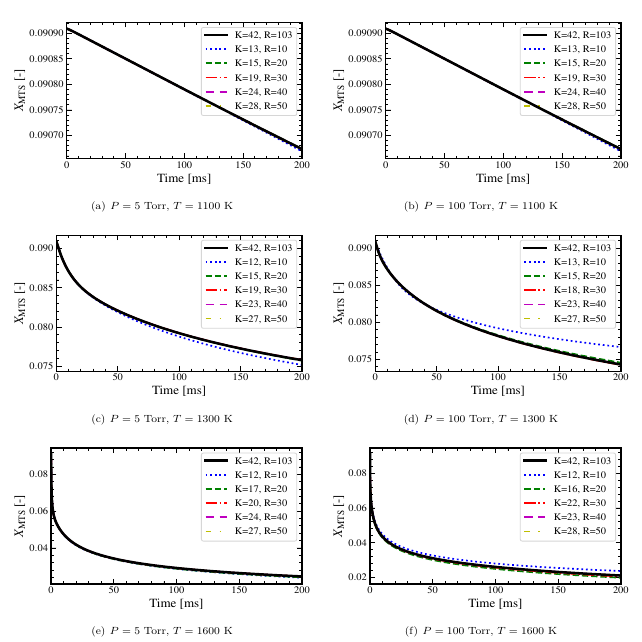
\includegraphics[width=\textwidth]{ph-fig2.png}
\caption{Comparison of time evolution of the mole fraction of MTS obtained using chemical mechanisms with different levels of complexity at T = 1100 K (a, b), T = 1300 K (c, d), and T = 1600 K (e, f) at P = 5 Torr (a, c, e) and P = 100 Torr (b, d, f). Here, K and R denotes the number of species and chemical reactions, respectively.}
\label{T-vs-t-MTS}
\end{figure}

\begin{figure}[p]
    \centering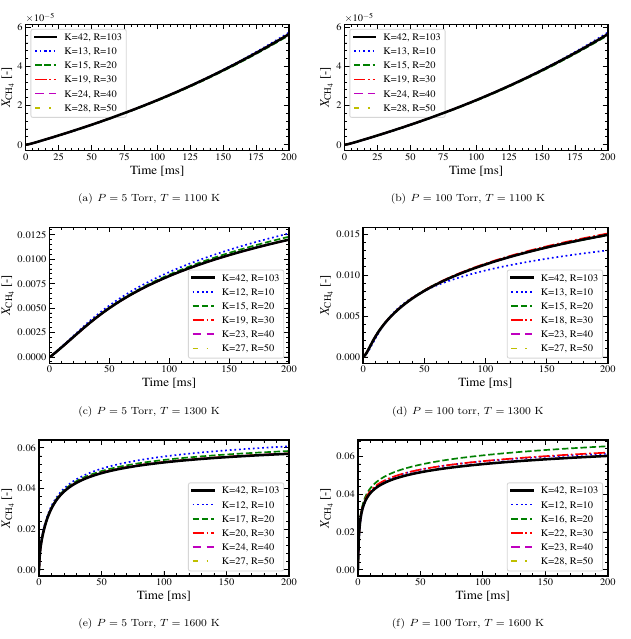
\includegraphics[width=\textwidth]{ph-fig3.png}
\caption{Comparison of time evolution of the mole fraction of CH$_4$ obtained using chemical mechanisms with different levels of complexity at T = 1100 K (a, b), T = 1300 K (c, d), and T = 1600 K (e, f) at P = 5 Torr (a, c, e) and P = 100 Torr (b, d, f). Here, K and R denotes the number of species and chemical reactions, respectively.}
\label{T-vs-t-CH4}
\end{figure}

\begin{figure}[tp] % FIXME: positioning of figures
    \centering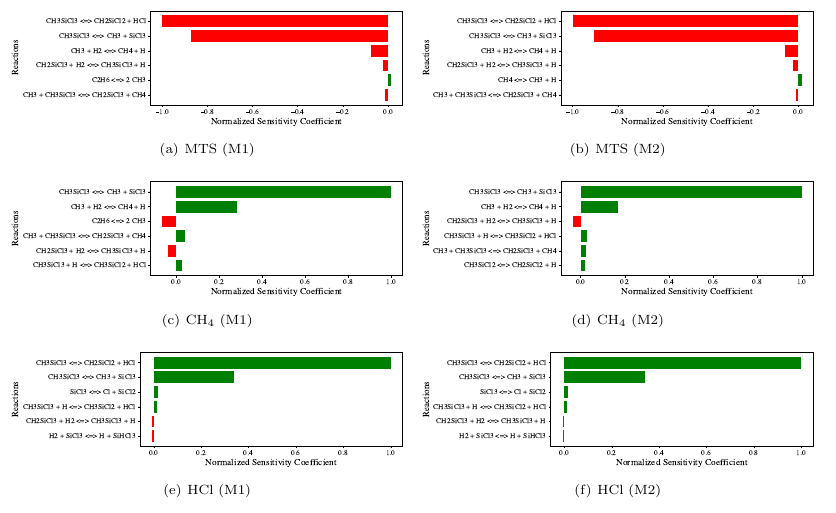
\includegraphics[width=\textwidth]{ph-fig4.png}
\caption{Six dominant reactions for MTS (a, b), CH$_4$ (c, d), and HCl (e, f) obtained using sensitivity analysis with M1 and M2 mechanisms.}
\label{Reactions-MTS-CH4-HCl}
\end{figure}

To further examine the dominant reactions corresponding to different species while using M1 and M2 mechanisms, a sensitivity analysis for different species is performed. The results from this analysis are shown in Fig. \ref{Reactions-MTS-CH4-HCl} for MTS, CH$_4$ , and HCl. With both M1 and M2 mechanisms, the three dominant reactions are the same, which are given by
\begin{align} %FIXME: tags in original are not right aligned like these are
    \rm CH_3SiCl_3 \leftrightarrow CH_2SiCl_2 + HCl, & \tag{R1} \\
    \rm CH_3SiCl_3 \leftrightarrow CH_3 + SiCl_3, & \tag{R2} \\
    \rm CH_3 + H_2 \leftrightarrow CH_4 + H, & \tag{R3}
\end{align}

\noindent Out of these three reactions, MTS is more sensitive to R1 and R2. These reactions play a critical role in the decomposition of MTS and leads to formation of reactive intermediates such as $\rm CH_2SiCl_2$, CH$_3$, and SiCl$_3$, which can further decompose, combine, or participate in heterogeneous surface reactions. Additionally, R1 also leads to HCl, which is a byproduct responsible for gas-phase etching \cite{Wang2008,Guan2020}. The R3 reaction is primarily responsible for the formation of CH$_4$, which can help avoid contamination, and the radical H, which is crucial for the removal of Cl and the promotion of SiC growth through heterogeneous reactions \cite{Brennan1990}. 

For CH$_4$ , R1 and R3 are the first two dominant reactions (see Fig. \ref{Reactions-MTS-CH4-HCl}(c) and (d)), which are found in both M1 and M2 mechanisms. However, the third dominant reaction is different for CH$_4$ with M1 and M2 mechanisms. While the M1 mechanism shows the third dominant reaction to be decomposition of $\rm C_2H_6$ into CH$_3$ radical through the reaction
\begin{align*}
    \rm C_2H_6 \leftrightarrow 2CH_3,
\end{align*}
the M2 mechanism shows the third dominant reaction as:
\begin{align*}
    \rm CH_2SiCL_3 + H2 \leftrightarrow CH_3SiCl_3 + H.
\end{align*}
This difference could be due to the absence of $\rm C_2H_6$ in the M2 mechanism (see Table \ref{table:1}). Although the third dominant reaction for CH$_4$ differs for the M1 and M2 mechanisms, the sensitivity of the first two dominant reactions is much higher compared to the third reaction.

An important byproduct during the decomposition of MTS is HCl. With both M1 and M2 mechanisms, similar to MTS, R1 and R2 are the first two dominant reactions (see Fig. \ref{Reactions-MTS-CH4-HCl}(e) and (f)), whereas the third dominant reaction is
\begin{align*}
    \rm SiCl_3 \leftrightarrow SiCl_2 + Cl.
\end{align*}
This is an intermediate and critical reaction, as SiCl$_2$ is a direct precursor to SiC formation via heterogeneous reaction with H$_2$ or CH$_2$ at the surface \cite{Papasouliotis1994}. On the other hand, the radical Cl can either react with H$_2$, leading to the formation of HCl, which in turn can prevent the formation of the undesirable Cl-rich byproducts such as SiCl$_4$.

To summarize, the results discussed in this section from the adiabatic reactor simulations and sensitivity analysis demonstrate that the reduced M2 mechanism can be considered adequate to capture the key aspects of MTS decomposition in the presence of H$_2$ in comparison to the detailed M1 mechanism for the conditions relevant to this study.

\subsection{Computational Cost}
As the number of species and reactions tends to differ in the three chemical mechanisms, it is expected that the computational cost will differ. A key focus of the present work is to demonstrate that moderately complex chemical kinetics, such as the M2 mechanism, can yield accurate results, which in turn can be used with CFD simulations. Here, we assess the computational cost of the three mechanisms by simulating a PFR at a pressure of 5 Torr and a temperature of 1350 K. The computational cost comparison is shown in Table \ref{table:2}.

\begin{table}[t]
    \centering
    \caption{Comparison of computational cost for 1 PFR simulation using M1, M2, and M3 mechanisms.}
    \label{table:2}
    \begin{tabular}{ | c | c | c | }
        \hline
        Mechanism & Computational Cost [s] & Relative Cost [\%] \\
        \hline
        M1 & 10.4 & 100 \\
        M2 & 4.6 & 44.2 \\
        M3 & 2.7 & 26 \\
        \hline
    \end{tabular}
\end{table}

As expected, the computational cost of the M2 and M3 mechanisms is lower than the detailed M1 mechanism. The cost of M2 decreases primarily due to a decrease in the number of species compared to M1, from 42 to 20, with a much less impact of a decrease in the number of reactions. Note that mechanisms such as M2 can be used for CFD simulations, as mechanisms with 15-20 chemical species tend to be manageable while employing finite-rate kinetics. However, it should be noted that the cost of a CFD simulation, apart from including the kinetics cost, also includes the cost of computation of convective and diffusive fluxes, which can be comparable to or larger than the cost of kinetics compared to a PFR simulation. The cost of M3 does not linearly scale with the number of species, which can be associated with a reduced rate of convergence of the PFR simulation with the M1 mechanism.

\subsection{Verification and Validation}
\begin{figure}[t] % FIXME: only using placeholder graphics
    \centering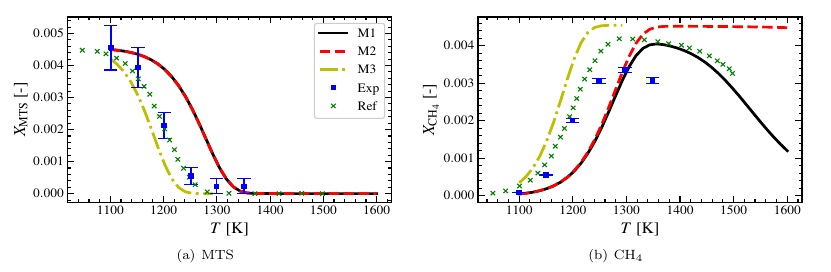
\includegraphics[width=\textwidth]{ph-fig5.png}
    \caption{Variation of mole fraction of MTS (a) and CH$_4$ (b) with respect to temperature. Experimental data and ‘Ref‘ data corresponds to experimental and computational study using detailed mechanism \cite{Dang2022}.}
\label{fig:5}
\end{figure}

We perform the verification and validation of the PFR-based strategy by simulating MTS decomposition in the presence of H$_2$ at an operating pressure of 1 atm (760 Torr), inlet composition ratio of 0.1, and over a range of temperatures varying from 1100 K to 1600 K. The results are compared in Fig. \ref{fig:5}, which includes the variation of the mole fraction of MTS and CH$_4$ with respect to temperature. For comparison, we also include experimental and computational results obtained using a detailed chemical mechanism from a past study \cite{Dang2022}. Note that the detailed mechanism used in the reference study was devised to match the experimental data. Furthermore, the operating pressure of the present configuration is much higher than that of a typical CVI, which is usually operated at lower pressures. 

Both M1 and M2 mechanisms yield the same results for MTS, which starts to decompose gradually from 1100 K to 1200 K, and then rapidly leads to a nearly complete decomposition by 1350 K. The values of MTS by these mechanisms are over-predicted compared to the reference results. Although the rate of decomposition of MTS from the M1 and M3 mechanisms matches during early and later stages with the reference computational results, the decomposition of MTS is delayed with respect to temperature. The results from the M3 mechanism are under-predicted compared to the reference results and show an early and faster rate of decomposition of MTS. Typically, one-step mechanisms, such as the M3 mechanism, are devised so that the variation of major species is captured well, which is not the case here, thus indicating its inaccuracy.

The results for the variation of CH4 mole fraction (see Fig. \ref{fig:5}(b)) from the M1 and M2 mechanisms tend to match till 1350 K. At temperatures beyond 1350 K, the M1 mechanism show reduced levels of CH$_4$ implying its further decomposition, whereas the M2 mechanism yields constant values of CH$_4$. The differences can be attributed to the effects of reduced number of species and reactions in the M2 mechanism compared to the M1 mechanism, which can affect the thermodynamics and reaction pathways. However, for typical CVI conditions of 800 to 1000 $^o$C, both mechanisms yield similar results, implying M2 can be considered to be accurate with respect to M1. As Fig. \ref{fig:5}(a) showed a delayed decomposition of MTS with respect to temperature using M1 and M2 mechanisms, this leads to a delayed production of CH$_4$ compared to the reference results. The peak value of CH$_4$ and its variation at higher temperatures by the M1 mechanism show good agreement with the reference computational results. Compared to experimental data, the peak values of CH$_4$ are over-predicted by all mechanisms. With the M3 mechanism, the production of CH$_4$ is over-predicted as it correlates with the under-prediction of MTS in Fig. \ref{fig:5}(a).

The results shown here demonstrate that the PFR strategy employed here can capture the decomposition of MTS in the presence of H$_2$. There are differences in the results from the detailed M1 mechanism and the detailed mechanism proposed in the reference study \cite{Dang2022}, which was devised to capture the experimental results. However, these differences are associated with a delayed start of decomposition of MTS and pro- duction of CH$_4$ with respect to temperature, although the rates of decomposition of MTS and production of CH$_4$ tend to match. In this study, we have not made any attempts to modify the baseline M1 mechanism, as the experimental data is only available at 760 Torr, whereas this study examines CVI reactor configurations at lower pressures. Therefore, the results from the M1 mechanism are considered as a reference in the rest of this study to examine the effects of operating conditions on the MTS decomposition and to assess the performance of the M2 and M3 mechanisms.

\section*{Acknowledgements}
This work was supported by the U.S. Department of Energy, Office of Science, Office of Basic Energy Sciences (BES), Gas Phase Chemical Physics (GPCP) through Grant \#DE-SC0024510.

%% References with bibTeX database:
\bibliographystyle{elsarticle-num}
\bibliography{cvi-bib}

\end{document}
